% Generated by documents/paper/figures/make_rq_appendix.py from the rq08_subset_selection README; do not edit.
\clearpage
\section{Subset selection}
\label{app:rq08_subset_selection}

\begin{rqfinding}
1. A chosen language subset beats the random-subset null in 72 of the 181 swept (benchmark, size) cells (72 of the 163 with a positive raw gain), by more than 0.25 SNR in 47, led by HellaSwag (median +0.85 over six sizes), Global-MMLU RF (+0.74), Belebele RF (+0.54) and MultiBLiMP (+0.47). XStoryCloze, LAMBADA, XWinograd, XCOPA and the BPB family never beat it, and XNLI sits below it (median $-$0.26). (Figure~\ref{fig:app_rq08_subset_selection}.)

2. Without the null the lever looks universal: the best prefix beats the full set in 163 of the 181 Case-1 cells that have an SNR (median +0.68 SNR), but the null, which scores 163 cells, keeps only 72.

3. Accuracy and BPB families: 52 of 113 cells beat the null (23 benchmarks); bBPB twins: 20 of 50 (14 twins), on the finals-only twins of this refresh.
\end{rqfinding}

\paragraph{Question.} Per benchmark, does a subset of subtasks --- a subset of \emph{languages} in a multilingual family, or a subset of \emph{subjects} in MMLU, or a subset of individual \emph{items} --- give higher SNR than the full set, and does the same subset hold across seeds and scales?

\paragraph{Setup.} Seed-1904 runs of every cell, 90M--1.7B; per multilingual benchmark and size, the language subset with the highest SNR (best prefix of languages ranked by SNR) against the 95th percentile of 100 random subsets of the same size; each per-language task gated above chance.

\begin{figure}[h]
\centering
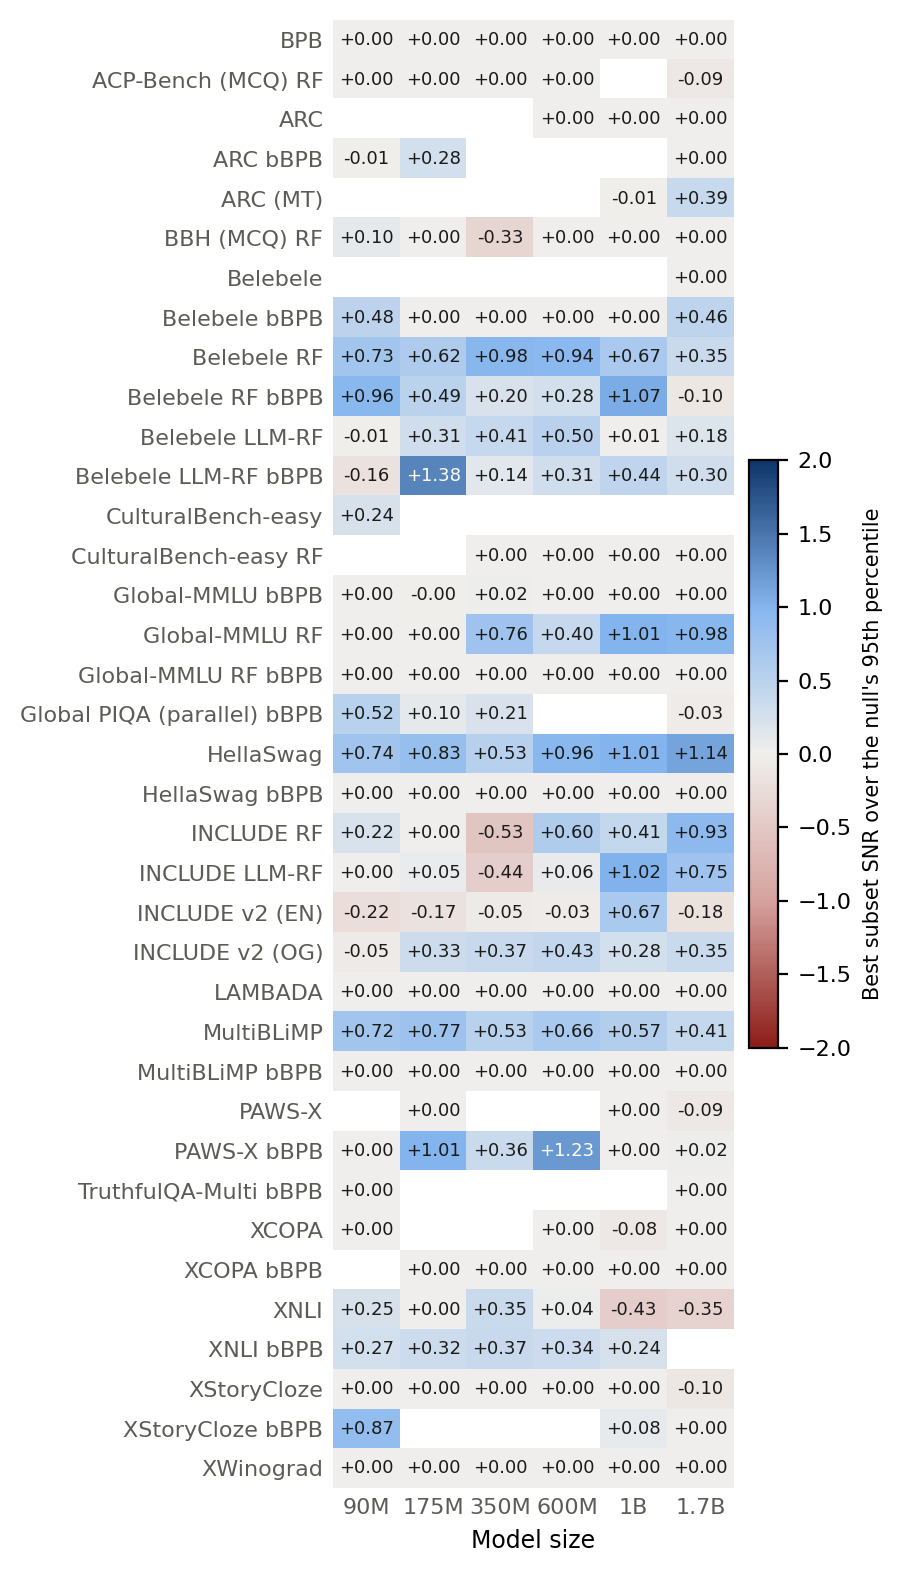
\includegraphics[width=\textwidth]{figures/app_subset_selection.png}
% source: src/signal-and-noise/analysis/rq08_subset_selection/pretraining/predictivity/gain_over_null_paper.png
\caption{Best language subset against the random-subset null, per benchmark and size.}
\label{fig:app_rq08_subset_selection}
\end{figure}
